\chapter{Desenvolvimento e Implementação}
Neste capítulo, apresenta-se a materialização do modelo proposto mediante a execução de uma Prova de Conceito (PoC). O propósito central consiste em evidenciar a viabilidade técnica da convergência entre os paradigmas de DevSecOps e a Infraestrutura como Código (IaC), fundamentando-se na estratégia de Shift-left. Esta abordagem visa a transposição dos controles de segurança para as fases embrionárias do ciclo de vida de desenvolvimento de software (SDLC), garantindo que a conformidade e a resiliência da infraestrutura sejam estabelecidas de forma nativa e automatizada, mitigando riscos antes mesmo do provisionamento dos recursos em ambiente de nuvem.

A validação prática do modelo proposto também foi realizada por meio de uma versão local da Prova de Conceito feita com Containers, descrita detalhadamente no Apêndice~\ref{apendice:poc-devsecops}.

\section{Cenário de Estudo: Prova de Conceito (PoC)}
Para a validação do modelo proposto, estruturou-se um ambiente de infraestrutura em nuvem pública utilizando a plataforma Amazon Web Services (AWS), com o Terraform atuando como motor de orquestração e provisionamento declarativo. A arquitetura da PoC concentrou-se em recursos críticos que, historicamente, apresentam elevados índices de configurações inseguras e vulnerabilidades em ambientes produtivos, conforme apontam os relatórios de conformidade do \citeonline{CIS2024AWS}:
\begin{itemize}
    \item\textbf{Instância de Computação (EC2):} Instâncias de computação configuradas para simular servidores de aplicação, permitindo a validação de regras de acesso e exposição de portas.
    \item\textbf{Armazenamento de Objetos (S3):} Baldes de armazenamento de objetos destinados à guarda de artefatos e logs, servindo como alvo para testes de criptografia em repouso e políticas de acesso público.
    \item\textbf{Camada de Rede e Acesso:} Implementação de Security Groups (firewall de rede) e Políticas de IAM (Identity and Access Management), essenciais para validar o princípio do privilégio mínimo e o controle de tráfego leste-oeste e norte-sul.
\end{itemize}

\section{Descrição do Ecossistema Tecnológico}
Para a viabilização da Prova de Conceito, selecionou-se um conjunto de ferramentas líderes de mercado que permitem a automação e a segurança nativa. Abaixo, detalham-se as tecnologias empregadas e suas respectivas funções na arquitetura:
\begin{itemize}
    \item\textbf{AWS (Amazon Web Services)} Provedor de computação em nuvem utilizado como ambiente de destino para a infraestrutura \citeonline{AWS2026}. Fornece a escalabilidade e os serviços (EC2, S3, IAM) cujas configurações de segurança foram o objeto central dos testes de conformidade.
    \item\textbf{Terraform (HashiCorp):} Ferramenta de Infraestrutura como Código (IaC) do tipo declarativa \citeonline{Terraform2026}. Utilizada para definir e provisionar os recursos da AWS por meio de arquivos de configuração, permitindo que a infraestrutura seja versionada e auditada como qualquer outro software.
    \item\textbf{Git e GitHub:} O Git foi utilizado para o controle de versão distribuído, permitindo o rastreio de alterações no código. O GitHub atua como o repositório central e plataforma de colaboração, onde gatilhos (hooks) de automação podem ser configurados \citeonline{Github2026}.
    \item\textbf{Checkov (Bridgecrew):} Ferramenta de análise estática (SAST) específica para infraestrutura \citeonline{Checkov2026}. Sua função na esteira é escanear os planos de execução e arquivos do Terraform em busca de configurações que violem boas práticas de segurança, como buckets abertos ou falta de criptografia .
    \item\textbf{GitGuardian:} Plataforma de detecção de segredos focada na prevenção de vazamento de credenciais. Atua monitorando commits em tempo real para identificar chaves de API, senhas ou tokens que possam ter sido inseridos acidentalmente no código \citeonline{GitGuardian2024}.
    \item\textbf{Open Policy Agent (OPA)} Motor de políticas de propósito geral que utiliza a linguagem Rego. No projeto, o OPA complementa o Checkov ao permitir a criação de regras customizadas de governança e controle financeiro (FinOps).
    
\end{itemize}

A organização do código-fonte foi estabelecida sob uma estrutura estritamente modular, fundamentada nos princípios de alta coesão e baixo acoplamento. Esta abordagem visa não apenas a reutilização de componentes em diferentes ambientes (como desenvolvimento, homologação e produção), mas, primordialmente, a segregação de responsabilidades (Separation of Concerns). Em vez de um arquivo de configuração monolítico, que dificultaria a rastreabilidade de falhas e a gestão de mudanças, cada elemento da infraestrutura definido na Prova de Conceito (PoC) foi isolado em diretórios e módulos específicos.

As camadas fundamentais de rede, computação e armazenamento foram dissociadas para permitir que cada uma possua seu próprio ciclo de vida e estado (state). Essa granularidade facilita a manutenção do código, pois permite que alterações em um componente de rede, por exemplo, sejam validadas e aplicadas sem impactar diretamente os recursos de computação, a menos que haja uma dependência explícita.

Sob a ótica da segurança, a modularização é o que viabiliza a aplicação de políticas granulares. Ferramentas de conformidade e análise estática, como o Checkov e o OPA, podem ser configuradas para realizar varreduras em escopos delimitados. Isso significa que é possível aplicar regras de conformidade mais rigorosas para o módulo de armazenamento (S3), exigindo criptografia mandatória e bloqueio de acesso público, enquanto o módulo de computação (EC2) é submetido a inspeções focadas em grupos de segurança e privilégios de identidade (IAM).

Além disso, a estrutura modular favorece a auditoria e a governança, uma vez que cada módulo pode ter proprietários definidos e permissões de acesso específicas no sistema de controle de versão. Essa organização é, portanto, o alicerce técnico que permite que a estratégia de Shift-left seja executada com precisão, garantindo que cada "peça" da infraestrutura nasça em conformidade com os padrões de segurança estabelecidos antes de sua integração ao ecossistema completo.

A Figura 3 apresenta o ambiente de desenvolvimento utilizado, destacando a estrutura de diretórios do projeto e a definição declarativa da Virtual Private Cloud (VPC).

\begin{figure}[ht]
    \caption{ Estrutura de diretórios e definição do módulo de rede (VPC) no Terraform, evidenciando a organização modular do projeto em ambiente WSL2 e o uso de boas práticas de parametrização para garantir a reutilização e a aplicação de políticas de segurança granulares. }
    \label{fig:cvss}
    \centering
    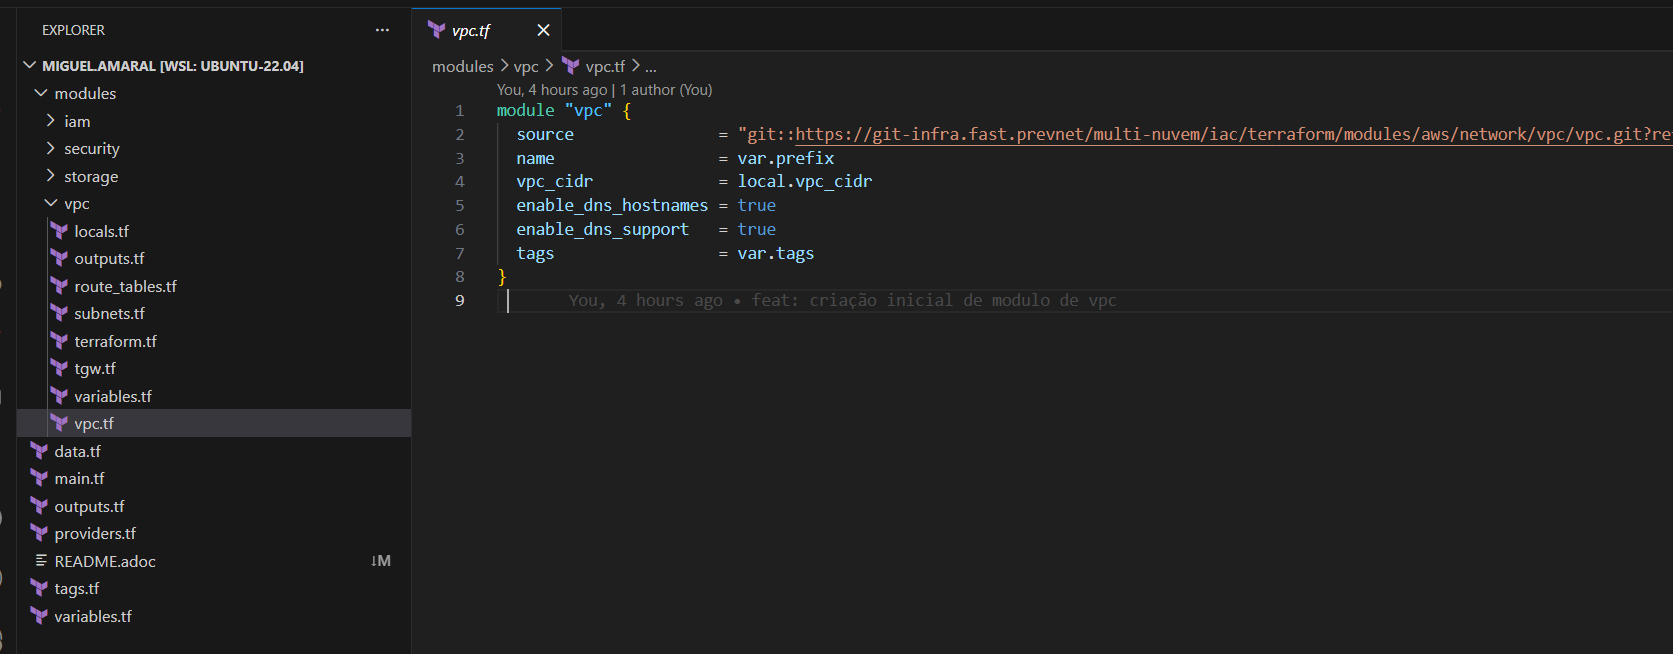
\includegraphics[width=0.8\textwidth]{Arquivos/figuras/Figura_Terraform_VPC.png}
    \fonte{Elaborado pelo autor}
\end{figure}

Conforme evidenciado na Figura 3, o projeto utiliza o IDE VS Code em um ambiente WSL2 (Ubuntu 22.04), refletindo uma stack padrão na engenharia de infraestrutura moderna. No explorador de arquivos, nota-se a divisão por módulos (iam, security, storage, vpc), o que possibilita que ferramentas como Checkov e OPA realizem varreduras em escopos delimitados de recursos. O arquivo \begin{foo}vpc.tf\end{foo}
ilustra a chamada de um módulo remoto via Git, empregando boas práticas de desenvolvimento, como a parametrização por variáveis (var.prefix, var.tags) e o uso de variáveis locais para o gerenciamento dinâmico de blocos de IP(\begin{foo}local.vpc_cidr\end{foo}
).

Esta organização é fundamental para a estratégia de Shift-left, pois permite que as verificações de segurança sejam executadas localmente pelo desenvolvedor — por meio de Pre-commit Hooks — antes mesmo do código ser enviado ao repositório central.

\section{ Arquitetura da Esteira DevSecOps e Detecção de Segredos}
A implementação do modelo seguiu o paradigma de Integração Contínua (CI), no qual cada alteração no código de infraestrutura desencadeia, de forma automatizada, uma série de validações hierárquicas de segurança. Nesse fluxo, o GitGuardian foi incorporado como um componente crítico para a operacionalização da Prevenção de Vazamento de Segredos (Secrets Detection). Esta ferramenta atua como um sentinela persistente, analisando cada commit em busca de padrões que indiquem a presença de credenciais sensíveis antes que estas sejam persistidas no histórico do projeto.

Diferente das ferramentas de análise de configuração, o GitGuardian especializa-se na identificação proativa de informações sensíveis expostas — como chaves de API da AWS, certificados digitais e credenciais de bancos de dados — que poderiam ser inadvertidamente incluídas no histórico do GitHub, utilizado nesta pesquisa como o sistema de controle de versão (VCS). A detecção precoce desses ativos é fundamental, pois uma vez que um segredo é enviado ao repositório, sua invalidação e a limpeza do histórico do Git tornam-se processos complexos e onerosos. Mesmo que o código seja removido em um commit posterior, o segredo permanece acessível no histórico de revisões, exigindo a revogação imediata da credencial para mitigar riscos de exploração.

Além da detecção técnica, a integração desta ferramenta promove uma mudança cultural no desenvolvimento da infraestrutura, estabelecendo uma "malha de segurança" que educa o desenvolvedor em tempo real. Ao receber um feedback imediato sobre a exposição de um segredo, a equipe de engenharia é instigada a adotar práticas mais seguras, como o uso de gerenciadores de segredos (Secret Managers) e variáveis de ambiente cifradas. Esse mecanismo de resposta rápida reduz drasticamente o TTD (Time to Detect), impedindo que vulnerabilidades de identidade, frequentemente exploradas em ataques de movimento lateral, sejam propagadas para ambientes produtivos.

A operacionalização do modelo proposto exige que a segurança seja integrada em todas as etapas do ciclo de vida de desenvolvimento (SDLC), estabelecendo uma barreira contínua do código-fonte até a produção. A Figura 4 ilustra a arquitetura da esteira DevSecOps implementada, detalhando a progressão do código entre os ambientes de construção (Build), homologação (Staging) e produção. Observa-se, por meio desta arquitetura, a atuação dos controles de segurança — como SAST, SCA e DAST — que funcionam como portões de qualidade (quality gates) indispensáveis para garantir a integridade e a resiliência da infraestrutura provisionada.

\begin{figure}[ht]
    \caption{ Diagrama de arquitetura da esteira DevSecOps integrada, detalhando o fluxo de trabalho desde o código-fonte até o ambiente de nuvem, destacando os portões de validação (SAST, SCA e Secrets Detection) que atuam como barreiras de conformidade. }
    \label{fig:cvss}
    \centering
    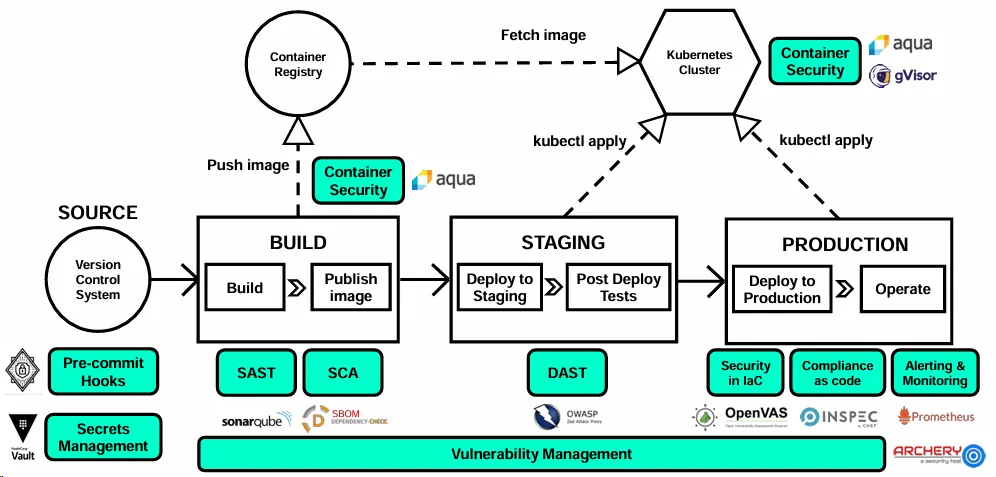
\includegraphics[width=0.8\textwidth]{Arquivos/figuras/Figura_Arquitetura_DevSecOps.png}
    \fonte{Elaborado pelo autor}
\end{figure}

Como observado no diagrama da Figura 4, a arquitetura foca na visibilidade total da vulnerabilidade. No início do fluxo (Source), destacam-se os Pre-commit Hooks e a gestão de segredos (Secrets Management), que impedem a propagação de credenciais sensíveis. Durante o Build, a análise estática (SAST) e a análise de composição de software (SCA) garantem a integridade das bibliotecas e do código IaC, enquanto a segurança de contêineres e o monitoramento contínuo fecham o ciclo no ambiente de execução, garantindo uma infraestrutura resiliente e auditável.

\subsection{Fluxo de Trabalho do GitGuardian}
O GitGuardian foi integrado em dois momentos distintos:
\begin{itemize}
    \item\textbf{Pre-commit Hooks:} Execução local na máquina do desenvolvedor para impedir que o commit seja realizado caso segredos sejam detectados.
    \item\textbf{Monitoramento do Repositório (Server-side):} Varredura contínua do histórico de commits no GitHub/GitLab para identificar segredos "vivos" que possam ter sido expostos anteriormente.
\end{itemize}



\section{Implementação das Verificações de Segurança com Checkov}
Após a validação de segredos, o código é submetido ao Checkov, uma ferramenta de Análise Estática de Segurança (SAST) específica para IaC. O Checkov avalia os arquivos .tf (Terraform) comparando-os com centenas de políticas pré-configuradas baseadas no framework CIS Benchmarks e melhores práticas da AWS.

Os principais controles implementados na PoC incluíram:

\begin{itemize}
    \item\textbf{Criptografia em repouso:} Validação obrigatória do parâmetro abaixo em baldes S3:
    \begin{foo}server_side_encryption_configuration\end{foo} 
    \item\textbf{Privilégio Mínimo:} Bloqueio de regras de entrada que utilizam o CIDR \begin{foo}0.0.0.0/0\end{foo} 
    em portas sensíveis (22, 3389 e 5432).
    \item\textbf{Imutabilidade e Registro:} Verificação de que o versionamento de objetos no S3 e o CloudTrail estão ativos para fins de auditoria forense.
\end{itemize}

A eficácia da análise estática depende da seleção rigorosa de políticas que reflitam os riscos reais do ambiente de nuvem. No âmbito desta Prova de Conceito, o Checkov foi configurado para atuar como uma barreira de qualidade (quality gate), comparando as definições do Terraform com um conjunto de regras preestabelecidas. A Tabela 1 detalha a matriz de políticas de segurança selecionadas para este estudo, correlacionando o recurso AWS afetado, o identificador da regra na ferramenta e a severidade atribuída à falha, conforme os padrões de conformidade do CIS Benchmarks.

\begin{table}[ht]
    \caption{ Matriz de políticas de segurança e conformidade configuradas no Checkov, correlacionando os recursos da infraestrutura AWS aos identificadores de regras baseados no framework CIS Benchmarks, detalhando a severidade de cada falha e os critérios de interrupção (Fail-Fast) adotados no ciclo de desenvolvimento. }
    \label{fig:cvss}
    \centering
    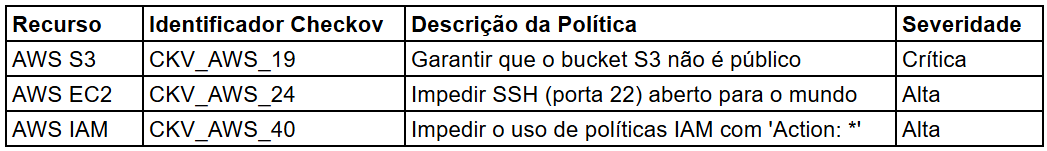
\includegraphics[width=0.8\textwidth]{Arquivos/figuras/Tabela_Verificacoes_Seguranca_Checkov.png}
    \fonte{Elaborado pelo autor}
\end{table}

A escolha dessas políticas justifica-se pela alta incidência de exposição de dados e acessos indevidos em infraestruturas mal configuradas. Conforme observado na Tabela 1, priorizou-se o bloqueio de falhas de severidade 'Crítica' e 'Alta', como a exposição pública de buckets S3 e o acesso SSH irrestrito, que são vetores comuns de ataques de ransomware e exfiltração de dados. A integração dessa matriz diretamente no ciclo de desenvolvimento permite que o analista de infraestrutura identifique e corrija tais vulnerabilidades em tempo de escrita, antes mesmo que os recursos sejam instanciados no console da AWS.

\section{Governança e Compliance com Open Policy Agent (OPA)}
Para estender a segurança além dos padrões de mercado, utilizou-se o Open Policy Agent (OPA) por meio da linguagem Rego. Enquanto o Checkov foca em vulnerabilidades técnicas, o OPA foi configurado para aplicar regras de governança e controle de custos (FinOps):

\begin{itemize}
    \item\textbf{Restrição de Instâncias:} Bloqueio do provisionamento de famílias de instâncias de alto custo (ex: \begin{foo}p3.2xlarge\end{foo}
    ) em ambientes de desenvolvimento (Tag: \begin{foo}Env = Dev\end{foo}
    ).
    \item\textbf{Whitelisting de Regiões:} Restrição do deploy apenas para a região \begin{foo}us-east-1\end{foo}
    , evitando recursos dispersos geograficamente que dificultam a conformidade com a LGPD.
\end{itemize}

\section{Ciclo de Feedback e Interrupção do Pipeline (Fail-Fast)}
O modelo implementado segue o princípio Fail-Fast. Se o GitGuardian detectar uma chave exposta ou o Checkov identificar uma falha crítica de segurança, o pipeline de CI/CD é interrompido imediatamente (Broken Build). O desenvolvedor recebe um feedback detalhado no console do terminal e na interface do Git, indicando o arquivo, a linha exata do erro e o link para a documentação de remediação.